\chapter{Week}
At the beginning of the week I held the second presentation 'Introduction to \ac{ML} on \acp{FPGA}' in front of the assembled engineering employees. At the end of the presentation a live demonstrator was shown at my work place. The ZCU 104 was used as the platform to show off all of the \ac{ML} examples provided by the \ac{DNNDK} and upcoming questions answered. The rest of the week was spent doing in depth research on integrating \ac{MIPI} into a Vivado block design. The reason for this is that Enclustra developed a new base board, the Mars ST3. This board features a \ac{MIPI} \ac{CSI} connector allowing high-speed video streaming with up to four lanes and a bit rate of 2.5 Gbit/s per lane (or 2.9 Gbit/s depending on the chosen clock rate). The camera chosen was the Raspberry Pi camera with a SONY image sensor. As \ac{MIPI} is not an open standard, research has been conducted into open source implementations of interfacing with the \ac{MIPI} protocol. After discussing the open source alternatives with more experienced employees, those solutions were deemed unsuitable for the task at hand. The alternative solution is to use a Xilinx \ac{IP} core which is available as a time limited evaluation license. The starting point was the ZCU 104 reference design, which included the whole \ac{MIPI} \ac{IP} core design. It consists of two main parts, the \ac{MIPI} D-PHY and the \ac{MIPI} Tx/Rx subsystem
\begin{figure}[!htb]
	\centering
		\includegraphics[width=\textwidth]{bilder/MIPI_dphy.png}
		\caption{D-PHY \acs{MIPI} \acs{IP} core overview~\cite{mipi-dphy}}
		\label{fig:mipi_dphy}
\end{figure}
A high-level view of the Xilinx \ac{MIPI} D-PHY \ac{IP} core system is shown in figure~\ref{fig:mipi_dphy}. The communication takes place between a Master and Slave with one clock lane and up to 4 data lanes. This \ac{IP} core allows proper communication on this high-speed I/O interface standard. The complete receiver subsystem is shown in figure~\ref{MIPI_rx}.
\begin{figure}[!htb]
	\centering
		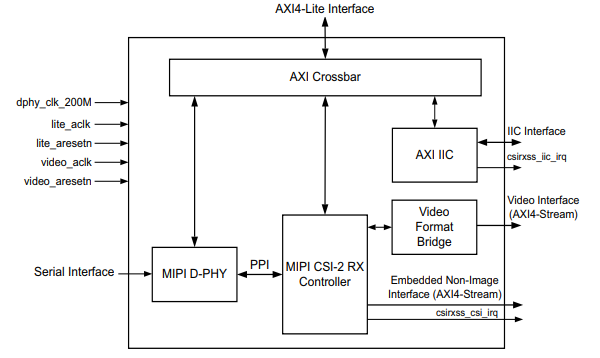
\includegraphics[width=\textwidth]{bilder/MIPI_rx.png}
		\caption{Receiver \acs{MIPI} \acs{IP} core subsystem~\cite{mipi-rx}}
		\label{fig:mipi_dphy}
\end{figure}
The D-PHY \ac{IP} core is part of this subsystem and in combination with the rest of the Rx subsystem allows the integration of a \ac{MIPI} based image sensor and an image sensor pipe. The captured images can then be accessed via \ac{AXI} interfaces. This part of the system needed to be integrated into the complete hardware design in Vivado consisting of the ZYNQ \ac{MPSoC}, the \ac{DPU} \ac{IP} core and the usual peripheral interfaces (\ac{USB}, DisplayPort, HDMI, etc.). On top of that, an embedded Linux \ac{OS} needed to be built to control the applications and provide a working demonstration environment. The chosen Linux distribution for this task was the Xilinx supported Petalinux, which is itself based on Yocto.